\documentclass[a4paper,12pt]{report}

\usepackage[vietnamese]{babel}
\usepackage[utf8]{inputenc, vietnam}
\usepackage[a4paper,margin=24mm]{geometry}
\usepackage[skip=10pt plus1pt, indent=20pt]{parskip}
\usepackage[colorlinks=true,allcolors=blue,urlcolor=magenta]{hyperref}

\usepackage{caption}
\usepackage{indentfirst,setspace,subcaption}
\usepackage{amsmath,amssymb,graphicx,xcolor,url}
\usepackage{fancyhdr,tocbasic,titlesec,minted,listings}

\renewcommand{\thesection}{\arabic{section}}

\renewcommand{\thesection}{\arabic{section}}
\renewcommand{\listoflistingscaption}{Source codes}

\newcommand{\codeimport}{\inputminted[breakanywhere=true,breaklines=true]}


% Code highlighting
\usemintedstyle{one-dark}
\setminted{frame=lines,
  framesep=2mm,
  baselinestretch=1.2,
  fontsize=\footnotesize,
  linenos,
  breakanywhere,
  breaklines,
  mathescape
}

% Header and footer styling
\pagestyle{fancy}
\setlength{\headheight}{18pt}
\fancyhf{}
\fancyhead[R]{\nouppercase\rightmark\hfill~Báo cáo đồ án OOP}
\fancyfoot[C]{\hfill\thepage\hfill}

% TOC styling
\DeclareTOCStyleEntry[
  indent=12pt,
  level=1
]{largetocline}{section}

% Title page data
\title{Báo cáo đồ án OOP}
\author{\begin{tabular}{r c}
  Ngô Nguyễn Thế Khoa & 23127065\\
  Phi Anh Khôi        & 23127073\\
  Khưu Ngọc Ý Vy      & 23127145\\
  Trần Phụng Đình     & 23127527\\
\end{tabular}}
\date{Ngày 1 tháng 11 năm 2024}

\begin{document}
\newenvironment{codewithlisting}[2]{
	\begin{listing}[!ht]
		\caption[#1]{#1}
		\label{listing:#2}}{\end{listing}
}

% Title page and TOC
\thispagestyle{empty}
\begin{titlepage}
	\begin{center}
		\makeatletter
		\newcommand{\HRule}{\rule{\linewidth}{0.4mm}}

		\textsc{\LARGE Đại học Quốc gia\\Thành phố Hồ Chí Minh}\\[1.5cm]
		\textsc{\Large Trường Đại học Khoa học Tự nhiên}\\[0.5cm]
		\textsc{\Large khoa công nghệ thông tin}\\[1.5cm]

		{\HRule}\\[1cm]
		{\huge \bfseries \@title}\\[0.5cm]
		{\HRule}\\[2cm]

		\textsc{\large CSC10003 -- Phương Pháp Lập Trình Hướng Đối Tượng}\\[0.5cm]

		\vfill\vfill\vfill

		{\large \@author}\\[1.5cm]
		{\large \@date}
		\makeatother
	\end{center}
\end{titlepage}

\tableofcontents\thispagestyle{empty}

% Report contents
\pagebreak
\section{Thông tin nhóm}
\begin{itemize}
  \item \textbf{Môn:} Phương pháp lập trình hướng đối tượng
  \item \textbf{Lớp học phần:} 23CLC09
  \item \textbf{Giảng viên hướng dẫn:} Bùi Tiến Lên
  \item \textbf{Thành viên:}
        \begin{center}
          \renewcommand{\arraystretch}{1.5}
          \begin{tabular}{|c|l|l|c|l|}
            \hline
            \textbf{STT} & \textbf{Họ và tên}  & \textbf{MSSV} & \textbf{Email}                                                       \\\hline
            1            & Ngô Nguyễn Thế Khoa & 23127065      & \href{mailto:nntkhoa23@clc.fitus.edu.vn}{nntkhoa23@clc.fitus.edu.vn} \\\hline
            2            & Phi Anh Khôi        & 23127073      & \href{mailto:pakhoi23@clc.fitus.edu.vn}{pakhoi23@clc.fitus.edu.vn}   \\\hline
            3            & Khưu Ngọc Ý Vy      & 23127145      & \href{mailto:knyvy23@clc.fitus.edu.vn}{knyvy23@clc.fitus.edu.vn}     \\\hline
            4            & Trần Phụng Đình     & 23127527      & \href{mailto:tpdinh23@clc.fitus.edu.vn}{tpdinh23@clc.fitus.edu.vn}   \\\hline
          \end{tabular}
        \end{center}
  \item \textbf{Công cụ hỗ trợ:}
        \begin{itemize}
          \item \href{https://git-scm.com/}{\textbf{Git}}, \href{https://github.com/}{\textbf{GitHub}}
          \item \href{https://docs.google.com/docs/}{\textbf{Google Docs}}
          \item \href{https://staruml.io/}{\textbf{StarUML}}
          \item \href{https://www.capcut.com/}{\textbf{CapCut}}
        \end{itemize}
\end{itemize}

\pagebreak
\section{Nội dung}
\subsection{Thông tin chung về đồ án:}
\begin{enumerate}
  \item \textbf{Tên đồ án:} Design Pattern
  \item \textbf{Môi trường lập trình:} Visual Studio Code
  \item \textbf{Ngôn ngữ lập trình:} C++
\end{enumerate}

% \pagebreak
\section{Bảng phân công việc}
\begin{center}
  \renewcommand{\arraystretch}{1.5}
  \begin{tabular}{|c|p{\dimexpr0.6\linewidth-2\tabcolsep}|c|}
    \hline
    \textbf{STT} & \textbf{Công việc} & \textbf{Người thực hiện} \\\hline
    1            & K                  & None                     \\\hline
    2            & K                  & None                     \\\hline
    3            & V                  & None                     \\\hline
    4            & D                  & None                     \\\hline
  \end{tabular}
\end{center}

\pagebreak
\section{Chi tiết về các Design Pattern được sử dụng}
\thispagestyle{empty}
\subsection{Pattern Name}
\subsubsection{Vấn đề}
\begin{flushleft}
	\begin{itemize}
		\item Ý 1
		\item Ý 2
	\end{itemize}

	\begin{enumerate}
		\item Ý 1
		\item Ý 2
	\end{enumerate}

	\begin{description}
		\item[Ý 1] Mô tả ý 1
		\item[Ý 2] Mô tả ý 2
	\end{description}
\end{flushleft}

\subsubsection{Mục đích}
\begin{flushleft}

\end{flushleft}

\subsubsection{Giải pháp}
\begin{flushleft}

\end{flushleft}

\subsubsection{Cấu trúc}
\begin{flushleft}

\end{flushleft}

\subsubsection{Khả năng ứng dụng}
\begin{flushleft}

\end{flushleft}

\subsubsection{Ưu nhược điểm}
\begin{flushleft}

\end{flushleft}
\thispagestyle{empty}
\subsection{Factory}
\subsubsection{Vấn đề}
\begin{flushleft}
	\begin{itemize}
		\item Ban đầu, hệ thống chỉ hỗ trợ thanh toán qua Credit Card và hoạt động hiệu quả, giúp tăng doanh thu và uy tín. Tuy nhiên, khi số lượng khách hàng tăng, cần đa dạng hóa hình thức thanh toán (Paypal, Stripe, v,v). 

		\item Việc này gặp khó khăn vì code hiện tại chỉ tập trung vào Credit Card, dẫn đến việc hệ thống trở nên phức tạp và khó quản lý khi thêm các hình thức thanh toán mới.
	\end{itemize}

	\begin{enumerate}
		\item Ý 1
		\item Ý 2
	\end{enumerate}

\end{flushleft}

\subsubsection{Mục đích}
\begin{flushleft}

\begin{itemize}
    \item Sử dụng Factory Pattern để cung cấp một giao diện ở lớp cha nhằm tạo ra những đối tượng nhưng vẫn cho phép những lớp con tùy chỉnh loại đối tượng được tạo ra. 

\end{itemize}



\end{flushleft}

\subsubsection{Giải pháp}
\begin{flushleft}

\begin{itemize}
    \item Chúng ta sẽ cài đặt một số phương thức ảo “Factory”. Thay vì tạo mới loại hình thanh toán một cách trực tiếp, giờ đây chúng ta sẽ tạo mới thông qua các phương thức ảo trên. 
    \item Điều này cho phép những loại hình thanh toán mới có thể được thêm vào hệ thống và điều chỉnh độc lập ở những lớp con thay vì phải điều chỉnh lại toàn bộ code của hệ thống. 
    \item Tuy nhiên ở lớp con cần phải tuân thủ trả về đầy đủ các kiểu trả về của Factory method đã được khai báo ở lớp cha. 
\end{itemize}

\end{flushleft}

\subsubsection{Cấu trúc}
\begin{flushleft}

    \begin{enumerate}
        \item Tạo một “Payment Interface” (hay còn gọi là một abstract class) với đầy đủ các tính chất và phương thức mà một giao dịch cần phải tuân theo. 
        \item Xây dựng những loại hình giao dịch cụ thể tuân theo Payment Interface trên (CreditCardPayment, PaypalPayment, StripePayment, v.v). 
        \item Ta cũng xây dựng một lớp “Creator” các loại giao dịch dưới dạng một abstract class để creator cho mỗi loại hình giao dịch khác nhau cũng phải tuân theo một số quy tắc được đặt ra của lớp creator trước đó. 
        \item Thực hiện các lớp creator đối với mỗi loại hình giao dịch được kế thừa từ lớp ảo creator trước đó trong mỗi lớp này sẽ gọi đến interface class của giao dịch để tạo ra loại hình giao dịch mà lớp này đang chịu trách nhiệm.

    \end{enumerate}

\end{flushleft}

\subsubsection{Khả năng ứng dụng}
\begin{flushleft}

\end{flushleft}

\subsubsection{Ưu nhược điểm}
\begin{flushleft}
    \begin{itemize}
        \item Ưu điểm
            \begin{itemize}
                \item Tránh những ảnh hưởng lẫn nhau giữa thành phần tạo ra đối tượng (creator) và các sản phẩm cụ thể (concrete product).
                \item Nguyên tắc trách nhiệm duy nhất: Tập trung mã tạo sản phẩm vào một nơi trong chương trình, giúp mã dễ dàng bảo trì hơn.
                \item Nguyên tắc Mở/Đóng: Bạn có thể thêm các loại sản phẩm mới vào chương trình mà không làm ảnh hưởng đến mã của các thành phần khác.
            \end{itemize}
        \item Nhược điểm
            \begin{itemize}
                \item Mã có thể trở nên phức tạp hơn vì cần tạo thêm nhiều lớp con mới để triển khai mẫu thiết kế.
            \end{itemize}
    \end{itemize}

\end{flushleft}
\subsection{Decorator}
\begin{flushleft}
    \textbf{Decorator} là một mẫu thiết kế cấu trúc cho phép mở rộng hoặc thêm chức năng mới cho một đối tượng động mà không làm thay đổi trực tiếp lớp của nó. `Decorator' hoạt động bằng cách bọc (wrap) đối tượng gốc, sau đó tùy chỉnh hoặc mở rộng hành vi của nó.
\end{flushleft}

\subsubsection{Vấn đề}
\begin{itemize}
    \item Hãy tưởng tượng bạn đang làm việc với một hệ thống xử lý đơn hàng thương mại điện tử. Ban đầu, hệ thống này rất đơn giản: mỗi đơn hàng chỉ chứa danh sách các sản phẩm và thông tin thanh toán cơ bản. Mọi thứ đều theo một quy trình mặc định, từ thanh toán đến vận chuyển tiêu chuẩn, không có tùy chọn bổ sung nào khác.
    \item Mọi thứ vẫn vận hành suôn sẻ cho tới khi khách hàng đưa ra các yêu cầu mới:
          \begin{itemize}
              \item \textit{`Tôi muốn đơn hàng được giao hỏa tốc vì tôi cần nó ngay bây giờ'}
              \item \textit{`Sản phẩm này là một món quà, hãy đóng gói thật đẹp giúp tôi'}
              \item \textit{`Hàng của tôi dễ vỡ, tôi muốn thêm bảo hiểm để đảm bảo an toàn'}
              \item \ldots
          \end{itemize}
    \item Bạn cố gắng cập nhật hệ thống để đáp ứng các yêu cầu này bằng cách thêm các thuộc tính mới vào lớp đơn hàng (như \textit{isGiftWrap, isExpressDelivery, hasInsurance\ldots}).\newline~Tuy nhiên điều này nhanh chóng trở nên phức tạp bởi vì:
          \begin{itemize}
              \item Mỗi yêu cầu bổ sung dẫn đến thêm nhiều điều kiện \textit{if-else} vào mã nguồn.
              \item Các phương thức xử lý đơn hàng trở nên cồng kềnh và khó bảo trì.
              \item Khi số lượng dịch vụ bổ sung tăng lên, việc tổ hợp các tùy chọn trở thành một cơn ác mộng.
          \end{itemize}
    \item Lúc này, bạn nhận ra cần một cách tiếp cận tốt hơn để mở rộng chức năng của đơn hàng mà không làm phức tạp thêm cấu trúc lớp gốc.
\end{itemize}

\subsubsection{Mục đích}
\begin{itemize}
    \item Để giải quyết vấn đề được đặt ra, bạn bắt đầu nghĩ đến kế thừa (Inheritance) để thay đổi lớp ban đầu. Tuy nhiên kế thừa lại có một số hạn chế như sau:
          \begin{itemize}
              \item \textbf{Tính chất tĩnh:} Hành vi được xác định tại thời điểm biên dịch, khó thay đổi khi chạy.
              \item \textbf{Không hỗ trợ đa kế thừa:} Nhiều ngôn ngữ lập trình không cho phép đa kế thừa, hạn chế khả năng mở rộng.
          \end{itemize}

    \item Bạn tiếp tục tìm đến những giải pháp khác là tập hợp (Aggregation) hoặc thành phần (Composition) để khắc phục nhược điểm của kế thừa:
          \begin{itemize}
              \item Cho phép đối tượng tham chiếu và ủy quyền nhiệm vụ cho các đối tượng khác.
              \item Thay đổi hành vi linh hoạt tại thời điểm chạy.
          \end{itemize}
    \item Hai nguyên tắc này nền tảng cho nhiều mẫu thiết kế, đặc biệt là \verb|Decorator Pattern|.
\end{itemize}

\subsubsection{Giải pháp}
\begin{enumerate}
    \item \textbf{Cơ chế của Decorator}\newline
          \textit{Decorator Pattern} mở rộng hành vi bằng cách `bọc' đối tượng trong các lớp mở rộng, mỗi lớp thêm hoặc thay đổi chức năng mà không ảnh hưởng đến đối tượng gốc.
          \begin{itemize}
              \item \textbf{Tham chiếu đối tượng gốc:} Các lớp Decorator chứa tham chiếu đến đối tượng cần bọc (có thể là đối tượng cơ bản hoặc một Decorator khác).
              \item \textbf{Giao diện thống nhất:} Decorator và đối tượng gốc tuân theo cùng một giao diện hoặc lớp trừu tượng. Điều này giúp Decorator có thể thay thế đối tượng gốc mà không làm thay đổi logic tổng thể.
              \item \textbf{Thêm hành vi từng bước:} Decorator thực hiện logic riêng trước hoặc sau khi gọi phương thức của đối tượng bọc.
              \item \textbf{Kết hợp các tính năng:}
                    \begin{itemize}
                        \item Đơn hàng cơ bản: sử dụng \textit{BasicOrder}.
                        \item Đơn hàng cần gói quà và vận chuyển nhanh: sử dụng \textit{GiftWrapDecorator} và \textit{ExpressDeliveryDecorator} bọc quanh \textit{BasicOrder}.
                    \end{itemize}
          \end{itemize}

    \item \textbf{Ứng dụng vào hệ thống xử lý đơn hàng}
          \begin{itemize}
              \item \textbf{Đối tượng cơ bản:} \textit{BasicOrder} là đơn hàng tiêu chuẩn, chỉ chứa thông tin sản phẩm, chi phí cơ bản và mã giảm giá.
              \item \textbf{Thêm Decorator theo yêu cầu:}
                    \begin{itemize}
                        \item \textit{GiftWrapDecorator}: Thêm phí và mô tả gói quà.
                        \item \textit{ExpressDeliveryDecorator}: Thêm phí và đơn vị giao hàng nhanh.
                    \end{itemize}
              \item \textbf{Xử lý tuần tự:} Khi gọi phương thức như \verb|calculateTotal()|, mỗi lớp Decorator sẽ thêm logic riêng, sau đó chuyển lời gọi tới lớp tiếp theo, tạo nên một luồng xử lý linh hoạt và có tổ chức.
          \end{itemize}
\end{enumerate}

\subsubsection{Cấu trúc}
\begin{flushleft}
    \begin{enumerate}
        \item \textbf{Order:} Đây là một giao diện (interface) xác định các hành vi cơ bản của một đơn hàng, bao gồm tính toán tổng tiền và đặt hàng.
        \item \textbf{BasicOrder:} Lớp cụ thể thực hiện giao diện \verb|Order|, đại diện cho một đơn hàng cơ bản. Lớp này có các thuộc tính như tổng giá trị giỏ hàng, mã giảm giá và các phương thức để tính toán tổng tiền và đặt hàng.
        \item \textbf{OrderDecorator:} Đây là một lớp trừu tượng (abstract class) đóng vai trò là lớp cơ sở cho các lớp `decorator'. Lớp này có một thuộc tính tham chiếu đến một đối tượng \verb|Order| khác (\verb|wrappedOrder|) và các phương thức để tính toán tổng tiền và đặt hàng. Các phương thức này thường sẽ gọi đến các phương thức tương ứng của \verb|wrappedOrder| và thực hiện thêm các logic của các `decorator' khác.
        \item \textbf{ExpressDeliveryDecorator:} Lớp cụ thể kế thừa từ \verb|OrderDecorator|, đại diện cho một lớp `decorator' thêm chức năng giao hàng nhanh cho đơn hàng. Lớp này có các thuộc tính như nhà cung cấp giao hàng, phí giao hàng và các phương thức để tính toán tổng tiền bao gồm cả phí giao hàng và cập nhật nhà cung cấp giao hàng.
    \end{enumerate}

    \begin{figure}[H]
        \centering
        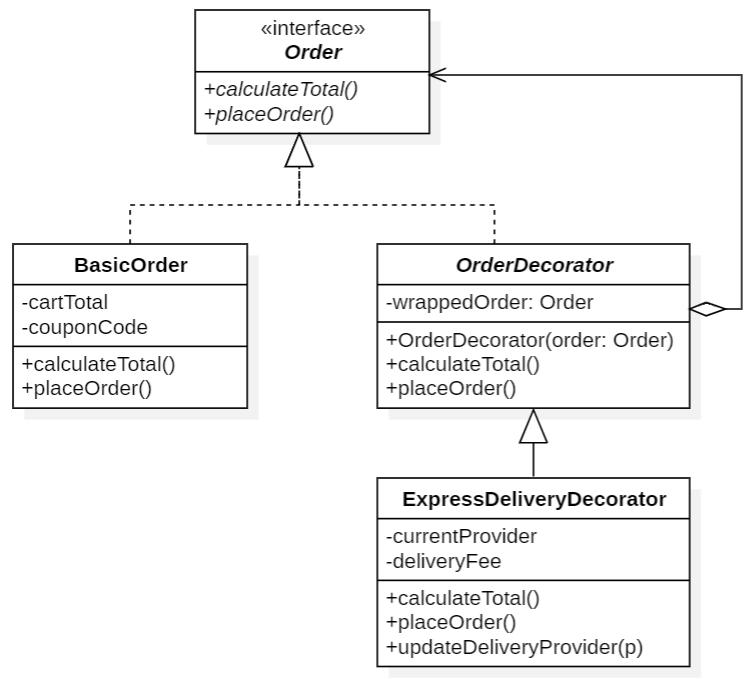
\includegraphics[width=0.9\textwidth]{../assets/screenshots/uml/decorator.png}
        \caption{Factory Method UML Class Diagram}
    \end{figure}
\end{flushleft}

\subsubsection{Hoạt động}
\begin{flushleft}
    \begin{itemize}
        \item \textbf{Tạo đối tượng BasicOrder:} Đầu tiên, chúng ta tạo một đối tượng \verb|BasicOrder| để đại diện cho một đơn hàng cơ bản.
        \item \textbf{Decorator:} Sau đó, chúng ta có thể tạo các đối tượng \verb|OrderDecorator| để `trang trí' cho đối tượng \verb|BasicOrder|. Ví dụ, chúng ta tạo một đối tượng \verb|ExpressDeliveryDecorator| và truyền đối tượng \verb|BasicOrder| vào trong constructor của nó.
        \item \textbf{Gọi phương thức:} Khi gọi các phương thức của đối tượng được trang trí (ví dụ: \verb|calculateTotal()|), các phương thức này sẽ gọi đến các phương thức tương ứng của đối tượng được gói bên trong (BasicOrder) và thực hiện thêm các logic trang trí. Trong trường hợp của \verb|ExpressDeliveryDecorator|, phương thức \verb|calculateTotal()| sẽ tính toán tổng tiền của đơn hàng cơ bản và cộng thêm phí giao hàng.
    \end{itemize}
\end{flushleft}

\subsubsection{Khả năng ứng dụng}
\begin{flushleft}
    \begin{itemize}
        \item \textbf{Tạo ra các loại đơn hàng đa dạng:}
              \begin{itemize}
                  \item \textbf{BasicOrder:} Đơn hàng tiêu chuẩn, chỉ chứa thông tin sản phẩm, chi phí cơ bản và mã giảm giá.
                  \item \textbf{ExpressDeliveryDecorator(BasicOrder):} Đơn hàng với giao hàng nhanh, có thêm phí và đơn vị giao hàng.
              \end{itemize}
        \item \textbf{Linh hoạt và mở rộng:} Để thêm một tính năng mới (ví dụ: gói quà), chỉ cần tạo một lớp decorator mới kế thừa từ OrderDecorator và triển khai logic thêm tính năng đó.
        \item \textbf{Tách biệt mối quan tâm:} Mỗi lớp decorator chỉ tập trung vào một tính năng cụ thể, giúp code dễ đọc, dễ bảo trì và dễ kiểm thử hơn.
    \end{itemize}
\end{flushleft}

\subsubsection{Ưu nhược điểm}
\begin{enumerate}
    \item \textbf{Ưu điểm}
          \begin{itemize}
              \item \textbf{Linh hoạt:} Dễ dàng thêm các tính năng mới cho một đối tượng mà không cần thay đổi lớp gốc.
              \item \textbf{Mở rộng:} Có thể kết hợp nhiều lớp trang trí để tạo ra các hành vi phức tạp.
              \item \textbf{Tái sử dụng:} Các lớp trang trí có thể được tái sử dụng cho nhiều loại đối tượng khác nhau.
          \end{itemize}
    \item \textbf{Nhược điểm}
          \begin{itemize}
              \item Việc loại bỏ một lớp Decorator cụ thể trong ngăn xếp không đơn giản.
              \item Hành vi của Decorator phụ thuộc vào thứ tự áp dụng.
              \item Việc có cấu trúc lớp phức tạp và khó khăn trong việc xác định hành vi của đối tượng khiến việc đọc hiểu mã nguồn trở nên khó khăn.
          \end{itemize}
\end{enumerate}

\subsubsection{Mã nguồn}
\codeimport{cpp}{../src/ecommerce-demo/Order.hpp}

\subsection{Chain of Responsibility}
\begin{flushleft}
	\textbf{Chain of Responsibility} là một mẫu thiết kế hành vi (behavioral design pattern) cho phép bạn truyền yêu cầu qua một chuỗi các bộ xử lý (handlers). Khi nhận được một yêu cầu, mỗi bộ xử lý sẽ quyết định hoặc xử lý yêu cầu đó hoặc chuyển nó cho bộ xử lý tiếp theo trong chuỗi.
\end{flushleft}

\subsubsection{Vấn đề}
\begin{flushleft}
	\begin{itemize}
		\item \textbf{Xử lý yêu cầu phức tạp:} Khi một yêu cầu cần được xử lý qua nhiều giai đoạn khác nhau, việc quản lý luồng xử lý và các điều kiện chuyển tiếp giữa các giai đoạn có thể trở nên phức tạp.
		\item \textbf{Mở rộng hệ thống:} Khi cần thêm hoặc xóa các giai đoạn xử lý, việc sửa đổi toàn bộ hệ thống có thể gây ra nhiều rắc rối.
		\item \textbf{Tách biệt mối quan tâm:} Các logic xử lý khác nhau được phân tán vào các lớp khác nhau, giúp code dễ đọc và bảo trì hơn.
	\end{itemize}
\end{flushleft}

\subsubsection{Mục đích}
\begin{flushleft}
	\begin{itemize}
		\item \textbf{Tách biệt các bước xử lý:} Mỗi bước xử lý được đóng gói trong một đối tượng riêng biệt (handler).
		\item \textbf{Xử lý theo chuỗi:} Các handler được liên kết thành một chuỗi, yêu cầu sẽ được truyền qua chuỗi cho đến khi được xử lý hoặc đạt đến cuối chuỗi.
		\item \textbf{Linh hoạt:} Dễ dàng thêm, xóa hoặc thay đổi thứ tự các handler mà không ảnh hưởng đến các phần còn lại của hệ thống.
	\end{itemize}
\end{flushleft}

\subsubsection{Giải pháp}
\begin{flushleft}
	\begin{itemize}
		\item Giống như nhiều mẫu thiết kế hành vi khác, \textit{Chain of Responsibility} dựa trên việc biến đổi các hành vi cụ thể thành các đối tượng độc lập gọi là \textit{handlers}.
		\item Mỗi công đoạn nên được trích xuất thành một lớp riêng biệt với một phương thức duy nhất thực hiện hành động cụ thể theo từng công đoạn. Yêu cầu, cùng với dữ liệu của nó, được truyền vào phương thức này như một đối số
		\item Mỗi handler được liên kết có một trường để lưu trữ tham chiếu đến handler tiếp theo trong chuỗi. Ngoài việc xử lý yêu cầu, các handlers còn truyền yêu cầu tiếp tục dọc theo chuỗi. Yêu cầu di chuyển dọc theo chuỗi cho đến khi tất cả các handlers đều có cơ hội xử lý nó.
	\end{itemize}
\end{flushleft}

\subsubsection{Cấu trúc}
\begin{flushleft}
	\begin{itemize}
		\item \textbf{OrderHandler:} Giao diện chung cho tất cả các handler, định nghĩa hai phương thức chính:
		      \begin{itemize}
			      \item \verb|setNext|: Thiết lập handler tiếp theo trong chuỗi.
			      \item \verb|handle|: Xử lý yêu cầu.
		      \end{itemize}
		\item \textbf{BaseHandler:} Lớp trừu tượng triển khai giao diện \verb|OrderHandler|, cung cấp một thuộc tính \verb|next| để lưu trữ handler tiếp theo.
		\item \textbf{SelectItemStage, AddressInfoStage, PaymentStage, ShippingStage, CompletionStage:} Các lớp cụ thể kế thừa từ \verb|BaseHandler|, đại diện cho các giai đoạn xử lý khác nhau trong một đơn hàng. Mỗi giai đoạn sẽ thực hiện một nhiệm vụ cụ thể và quyết định có chuyển yêu cầu đến giai đoạn tiếp theo hay không.
	\end{itemize}

    \begin{figure}[H]
        \centering
        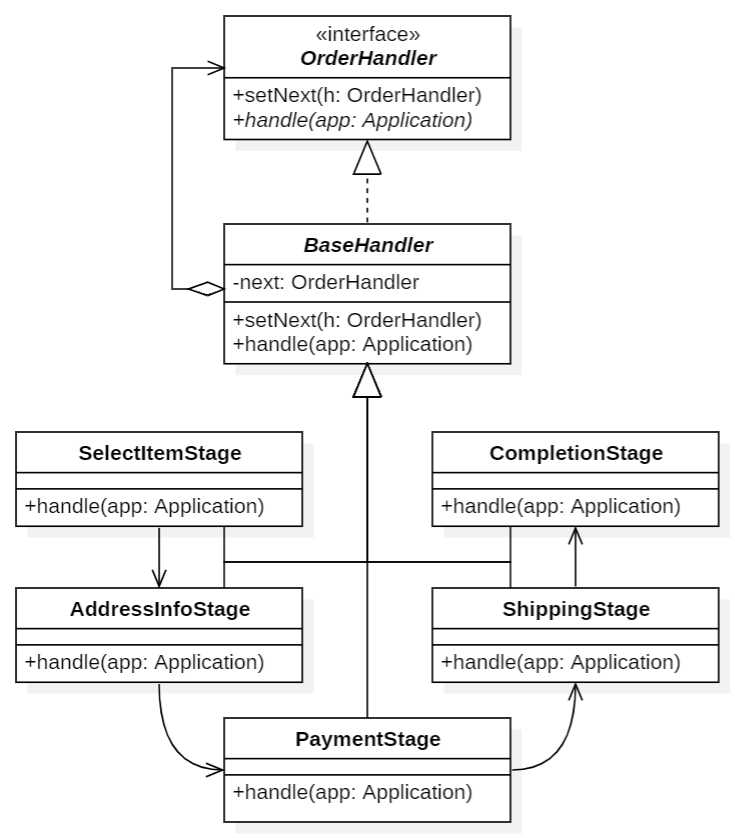
\includegraphics[width=0.9\textwidth]{../assets/screenshots/uml/cor.png}
        \caption{Chain of Responsibility UML Class Diagram}
    \end{figure}
\end{flushleft}

\subsubsection{Hoạt động}
\begin{flushleft}
	\begin{itemize}
		\item \textbf{Tạo chuỗi handler:} Các handler được khởi tạo và liên kết với nhau thành một chuỗi.
		\item \textbf{Gửi yêu cầu:} Yêu cầu được gửi đến handler đầu tiên trong chuỗi.
		\item \textbf{Xử lý yêu cầu:}
		      \begin{itemize}
			      \item Nếu handler hiện tại có thể xử lý yêu cầu, nó sẽ thực hiện các tác vụ cần thiết và dừng quá trình.
			      \item Nếu handler hiện tại không thể xử lý, nó sẽ chuyển yêu cầu đến handler tiếp theo trong chuỗi.
		      \end{itemize}
		\item \textbf{Lặp lại bước 3:} Quá trình này tiếp tục cho đến khi yêu cầu được xử lý hoặc đạt đến cuối chuỗi.
	\end{itemize}
\end{flushleft}

\subsubsection{Khả năng ứng dụng}
\begin{flushleft}
	\begin{itemize}
		\item \textbf{Xử lý đơn hàng:} \textit{CoR Pattern} được sử dụng rộng rãi trong các hệ thống xử lý đơn hàng để quản lý các giai đoạn khác nhau như thanh toán, vận chuyển.
		\item \textbf{Xử lý sự kiện:} Có thể sử dụng CoR để xử lý các sự kiện trong giao diện người dùng, chẳng hạn như các sự kiện click chuột để chuyển sang công đoạn kế.
		\item \textbf{Logging:} Mỗi handler có thể ghi lại thông tin về quá trình xử lý yêu cầu.
	\end{itemize}
\end{flushleft}

\subsubsection{Ưu nhược điểm}
\begin{enumerate}
	\item \textbf{Ưu điểm}
	      \begin{itemize}
		      \item \textbf{Linh hoạt:} Dễ dàng thêm, xóa hoặc thay đổi các handler.
		      \item \textbf{Mở rộng:} Có thể dễ dàng mở rộng hệ thống bằng cách thêm các handler mới.
		      \item \textbf{Tái sử dụng:} Các handler có thể được sử dụng lại trong các hệ thống khác.
		      \item \textbf{Giảm sự kết hợp:} Các handler không cần biết về các handler khác trong chuỗi.
	      \end{itemize}
	\item \textbf{Nhược điểm}
	      \begin{itemize}
		      \item \textbf{Khó phát hiện lỗi và debug:} Nếu chuỗi (chain) quá dài và phức tạp, việc tìm ra lỗi có thể khó khăn.
		      \item \textbf{Hiệu suất:} Nếu có quá nhiều handler, việc truyền yêu cầu qua chuỗi có thể làm giảm hiệu suất.
	      \end{itemize}
\end{enumerate}

\subsubsection{Mã nguồn}
\codeimport{cpp}{../src/ecommerce-demo/Stage.hpp}


\pagebreak
\section{Source}
\codeimport{cpp}{../src/ecommerce-demo/main.cpp}
\codeimport{cpp}{../src/ecommerce-demo/Payment.hpp}
\codeimport{cpp}{../src/ecommerce-demo/Order.hpp}
\codeimport{cpp}{../src/ecommerce-demo/Stage.hpp}

\pagebreak
\section{Ảnh chụp màn hình}
% \subsection{Demo}
% \begin{figure}[ht]
%   \centering
%   \includegraphics[width=0.7\textwidth]{Screenshots/server-console.png}
%   \caption{Giao diện Server (Console)}\label{fig:server-console}
% \end{figure}

% References
\pagebreak
\section{Nguồn tham khảo}
\begin{enumerate}
  \item \href{https://www.youtube.com/watch?v=oBykLn64AUc}{Class Diagram in UML}
\end{enumerate}

\end{document}